\begin{figure*}[t]
\centering
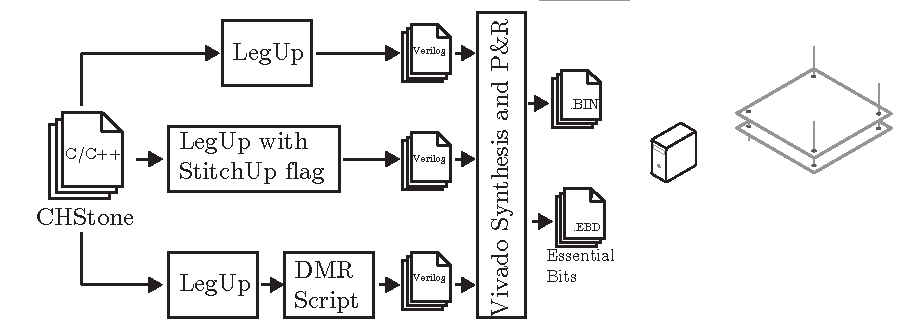
\includegraphics[width=6in]{./imgs/ExperimentFlow.pdf}
\caption{The experiment flow}
\label{fig:ExperimentFlow}
\end{figure*}

To test the error mitigation abilities of the circuits generation we are adopting the
gold standard of hardware fault injection, where configuration bits on the 
FPGA device are flipped from their original state.
Typical FPGA designs will require a large number of configuration bits, since this
memory is used to both program the functionality of the LUTs and the routing between
logic cells.
Traditionally random error injection is used since injection into every configuration
bit and re-running the circuit takes time, however we have developed an experiment
platform that allows us to achieve full exhaustive fault injection in reasonable time
and where possible we have used this to test StitchUp.

To achieve exhaustive testing we make use of many low cost Xilinx FPGA SoC devices known as
Zedboards, all injecting on the same circuit in parallel.
Multiple Zedboards, running Linux on the hardened ARM, are arranged into a cluster and
managed by a single desktop machine affectionatly called The SoC Drawer.

This approach was also made possible by the fact that the latest release of the LegUp tool
(v4.0) supports the generation of generic Verilog circuits, enabling it to be compiled
to Xilinx devices.
A Xilinx Soft Error Mitigation (SEM) IP Core connected to the FPGA internal configuration
port (ICAP) was responsible for flipping the configuration bits.
This was instantiated along with the StitchUp circuit and everything connected to the hard
ARM processing system via AXI interconnects.  
Software running under Linux on each of the ARM cores was then responsible, for sending the
address and injection command to the SEM core, starting the circuit under test, and
collecting the result from that circuit. 

Figure \ref{fig:ExperimentFlow} shows an overview of the experiment setup.
Each circuit at the top is fed into three different flows:
On the  left a full DMR version of the circuit is built, this uses LegUp to generate a 
single circuit and then wrapper scripts to connect them together and
generate comparison logic on the state register and output value;
in the middle a circuit is generated using the StitchUp flow, protecting only the control
structure of the original circuit; and on the right the original circuit with no protection
is produced via a standard LegUp pass.

Each different version is then passed through the Xilinx FPGA circuit tool flows to produce
two files, an essential bits file (.EBD), and a configuration binary (.BIN).
The essential bits file is a list of all the bits in the configuration memory that have any
influence on our generated circuit, and we use it to reduce the number of injections
required to fully test our design.

Both the EBD and BIN files are then sent to The SoC Drawer where they are allocated to
devices for testing, if they are small enough then they are allocated to run on the 
cluster of Zedboards where they will be exhaustively tested, while the larger circuits 
are allocated to a larger ZC706 device for random testing.
Designs allocated to the Zedboards have their EBD files divided up
into smaller chunks and each chunk is processed in parallel on a different Zedboard device.

\subsection{Performing the error injection}
Software responsible for each indivudal injection experiment injects a fault at the 
next consecutive address then runs the circuit storing the result.
If the circuit does not respond within three orders of magnitude of it's expected time
a timeout halts it and is recorded.
The fault is then repaired by re-injecting an error into the
same configuration memory location (i.e. flipping the bit back to it's original state)
and moves onto the next essential bit address.

The results are then analysed and each run is classified into three separate categories:

\begin{enumerate}
\setlength{\itemsep}{1pt}
\setlength{\parskip}{0pt}
\setlength{\parsep}{0pt}
\item Execution Time Error - This is where the execution of the circuit either took
an incorrect number of cycles to complete or timed out. Errors of these type are almost
always control flow related since any deviation from the correct execution path will cause
an incorrect number of cycles.
\item Data-Flow Only Errors - These are errors where the circuit has returned an incorrect
data result but has executed in the correct number of cycles, such error could be caused
by a non-control structure functional unit.
\item Caught Errors - These are errors that were detected by the protection method, which is
either DMR or StitchUp.
\end{enumerate}
